\documentclass{article}
\usepackage{graphicx}
\usepackage{float}
\usepackage{hyperref}
\usepackage[boxruled,vlined,linesnumbered]{algorithm2e}
\usepackage{amsmath}

\newcommand{\myparagraph}[1]{\paragraph{#1}\mbox{}}
\newcommand{\mysubparagraph}[1]{\subparagraph{#1}\mbox{}}

\begin{document}

\title{Logistic Regression and Neural Networks}
\author{William Grim \\ \href{mailto:grimwm@gmail.com}{grimwm@gmail.com}}

\maketitle

\tableofcontents

\begin{abstract}
For both logistic regression and neural networks, there are several common variables and equations between them.  Most of the time, the only difference between logistic regression, where mostly vectors are used, neural networks use matrices in their place for the multiple activation nodes.

This document will assume some knowledge of the Python library, \textbf{numpy} , which is introduced in the course in general.
\end{abstract}

\section{Logistic Regression}

\subsection{Variables and Definitions}

\begin{itemize}
\item $m$: number of training samples
\item $n_x$: number of features
\item $X = X_{n_x,m}$: a matrix with $m$ columns of training samples, each sample having $n_x$ features
\item $x^{(i)}$: an input sample column of data (e.g. pixels)
\item* $a = \hat{y} = \sigma(z)$: sigmoid or Rectified Linear Unit (RELU) function
\item $w = w_{n_x,1}$: an unknown parameter (vector) we are trying to learn
\item $b$: an unknown parameter (scalar) we are trying to learn
\item $\alpha$: learning rate
\end{itemize}

\subsection{Equation Cheat Sheet}

\begin{enumerate}
\item Linear function
$$z = w^T X + b$$
\item Activation function
$$a = \hat{y} = sigmoid(z) = \sigma(z) = \frac{1}{1 + e^{-z}}$$
\item Error or Loss function
$$L(a,y) = -\frac{1}{m} \sum_{i=1}^{m} (y\ log(a) + (1-y) log(1-a))$$
\item Cost function
$$J(a,y) = -\frac{1}{m} \sum_{i=1}^{m} L(a^{(i)},y^{(i)})$$
\item Cost with respect to weights
$$\frac{\partial{J}}{\partial{w}} = \frac{1}{m}X(A-Y)^{T}$$
\item Cost with respect to intercept
$$\frac{\partial{J}}{\partial{b}} = \frac{1}{m} \sum_{i=1}^{m}(a^{(i)} - y^{(i)})$$
\end{enumerate}

\subsection{Cost Analysis Function}

\subsubsection{Intuition}

In general, we want a formula meeting these requirements:

\begin{gather}
p(y=1|x) = a \\
p(y=0|x) = 1 - a
\end{gather}

As seen below, the following formula meets these requirements for $p(y | x)$:

Given:
$$p(y|x) = a^{y}(1-a)^{1-y}$$

Substituting $y=1$ or $y=0$, respectively:

\begin{gather}
p(y=1|x) = a^{1}(1-a)^{1-1} = a \\
p(y=0|x) = a^{0}(1-a)^{1-0} = 1-a
\end{gather}

\subsubsection{Error/Cost/Loss Function}

Applying the $log$ function to both sides of $p(y | x)$, we have

\begin{gather}
L(a,y) = log(p(y|x)) = log(a^{y}(1-a)^{1-y}) \\
= log(a)^y + log (1-a)^{1-y} \\
= y\ log(a) + (1-y) log (1-a)
\end{gather}

$L(a,y)$ is the amount of error between our predictions and the true values.  This is the case because $a$ comes from our predicted weights ($w$) multiplied by our input data ($X$) and passed to our activation function.  If we had no error, this loss function would be 0, meaning that if we predicted $w$ properly, then $y = a$ would be true.

\subsubsection{Minimize Our Cost}

Given the cost function above, as we optimize our predictions for $w$ and $b$, we want to minimize our costs, not maximize them; so, we must negate our cost.  Additionally, we want to perform the cost analysis for each activation, $a^{(i)}$ and take the average of all the costs. Therefore, we come to this solution:

$$J(a,y) = -\frac{1}{m} \sum_{i=1}^{m} L(a^{(i)},y^{(i)})$$

\subsubsection{Gradient Descent}

Finally, to optimize prediction parameters $w$ and $b$, we have to have the partial derivatives $\frac{\partial{J}}{\partial{w}}$ and $\frac{\partial{J}}{\partial{b}}$.  Before going into the derivations, here is some insight on how they are used when minimizing $J(a,y)$

\myparagraph{Numerical Gradient Descent Explained Graphically}

First, let's start with a view of a function $f(z)$ and its derivative, which is labeled $t(z)$:

\begin{figure}[H]
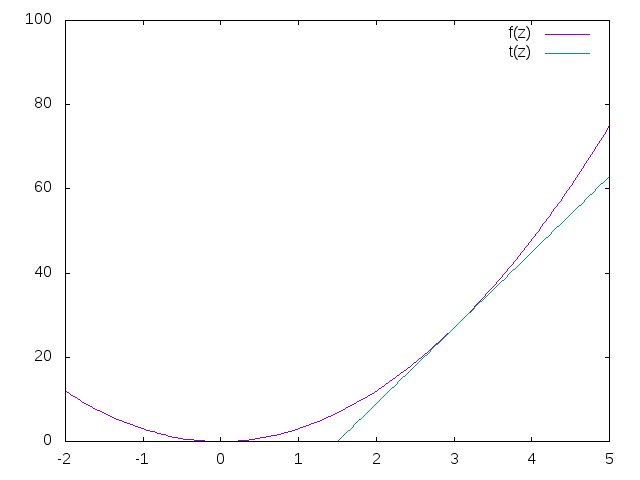
\includegraphics[width=\linewidth]{grad_descent.png}
\caption{Gradient Descent}
\label{fig:grad_descent}
\end{figure}

Our goal is to modify the input variable $z$ to minimize $f(z)$, and we can do this by minimizing $t(z)$, implying that we can minimize $f(z)$ by minimizing $z$.

Symbolically, the above is very simple using the standard rules of calculus.  However, when dealing with complex functions, we are forced to do iterative gradient descent numerically.  So, our approach will be as seen in Algorithm \ref{alg:z_update_rule}.

\begin{algorithm}[h]
\caption{Z Update Rule}
\label{alg:z_update_rule}
\For{i:=1 to N}{
z := z - $\alpha$ dz\;
dz := expected - f(z)\;
}
\end{algorithm}

Iteratively performing the above formula many times, updating our derivative each time will help us walk along the curve and find its minimum.  $\alpha$ is called the "learning rate" and allows us to walk along the curve faster or slower but also introduces error the larger it is.  Too small, however, and it might take too long to find $f(z)$'s optimum value.

\myparagraph{Partial Derivative $\frac{\partial{J}}{\partial{w}}$}

First, we will introduce the final formulas, and then we will break down the math into steps.

\mysubparagraph{Conclusions}

\begin{gather}
\frac{\partial{J}}{\partial{w}} = \frac{1}{m}X(A-Y)^{T} \\
%
\frac{\partial{J}}{\partial{b}} = \frac{1}{m} \sum_{i=1}^{m}(a^{(i)} - y^{(i)})
\end{gather}

\mysubparagraph{Partial Derivations}

\begin{gather}
\frac{\partial{J}}{\partial{w}} = \frac{\partial{J}}{\partial{L}}\frac{\partial{L}}{\partial{a}}\frac{\partial{a}}{\partial{z}}\frac{\partial{z}}{\partial{w}} \label{eqn:dJ_dw} \\
%
\frac{\partial{J}}{\partial{b}} = \frac{\partial{J}}{\partial{L}}\frac{\partial{L}}{\partial{a}}\frac{\partial{a}}{\partial{z}}\frac{\partial{z}}{\partial{b}} \label{eqn:dJ_db} \\
%
\frac{\partial{J}}{\partial{L}} = 1 \\
%
\frac{\partial{z}}{\partial{w}} = \frac{\partial{[w^T x + b]}}{\partial{w}} = x \\
%
\frac{\partial{z}}{\partial{b}} = \frac{\partial{[w^{T} x + b]}}{\partial{b}} = 1 \\
%
\frac{\partial{a}}{\partial{z}} = \frac{\partial{[\frac{1}{1 + e^{-z}}}]}{\partial{z}} = \frac{-e^{-z}}{(1+e^{-z})^{2}} \\
%
\frac{\partial{L}}{\partial{a}} = \frac{\partial{[y\ log(a) + (1-y) log (1-a)]}}{\partial{a}} \\
= \frac{y}{a} - \frac{1-y}{1-a} = \frac{y-ya-a+ya}{a(1-a)} \\
= \frac{a-y}{a(a-1)}
\end{gather}

\mysubparagraph{Substitutions}

Beginning with Equation \ref{eqn:dJ_dw}, we will now substitute all variables into place and simplify.

\begin{gather}
\frac{\partial{J}}{\partial{w}} = 1 * \frac{a-y}{a(a-1)} * \frac{e^{-z}}{(1+e^{-z})^{2}} * x \\
%
a = \sigma(z) = \frac{1}{1 + e^{-z}} \\
%
\frac{a-y}{a(a-1)} = \frac{\frac{1}{1 + e^{-z}} - y}{\frac{1}{1 + e^{-z}} \frac{-e^{-z}}{1 + e^{-z}}} = \frac{(1+e^{-z})^2 (\frac{1}{1 + e^{-z}} - y)}{-e^{-z}} \\
%
\frac{a-y}{a(a-1)} * \frac{-e^{-z}}{(1+e^{-z})^{2}} = a-y \\
%
\frac{\partial{J}}{\partial{w}} = x(a-y)
\end{gather}

Therefore, additionally solving for $\frac{\partial{J}}{\partial{b}}$, we end up with these two very important derivatives.

\begin{gather}
\frac{\partial{J}}{\partial{w}} = x(a-y) \\
%
\frac{\partial{J}}{\partial{b}} = a-y
\end{gather}

Expanding the two above equations to vectors and matrices with $m$ samples, we arrive at the final versions of the derivations that we will be using:

\begin{gather}
\frac{\partial{J}}{\partial{w}} = \frac{1}{m} X(A-Y)^{T} \\
%
\frac{\partial{J}}{\partial{b}} = \frac{1}{m} \sum_{i=1}^{m} (a^{(i)} - y^{(i)})
\end{gather}

In case it's not obvious why we do a summation in one of the forumlas and not the other, it is because the matrix multiplication already implies summations when it computes the dot products.  For the other formula, however, we are not performing matrix multiplication and must therefore do the summation ourselves.

\end{document}

